91. \begin{figure}[ht!]
\center{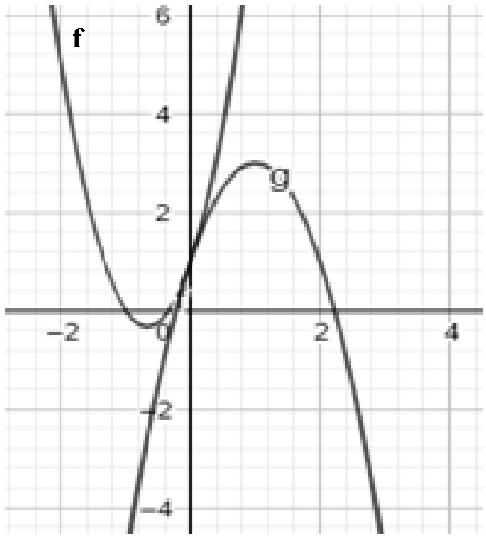
\includegraphics[scale=0.35]{grpar.png}}
\end{figure}\\
На рисунке параболы $f$ с уравнением $y=a_1 x^2+b_1x+c_1$ и $g$ с уравнением $y=a_2 x^2+b_2x+c_2$ касаются друг друга в точке, лежащей на оси ординат. Найдите соотношение между коэффициентами $a_1$ и $a_2;\ b_1$ и $b_2;\ c_1$ и $c_2.$\\
